\documentclass{beamer}
\usetheme{Boadilla}
\usepackage{tikz}
% \usepackage{enumitem}

\title{MTH 1030 Week 9 tutorial}
\author{Alex Elzenaar}

\newcommand{\R}{\mathbb{R}}

\begin{document}


\begin{frame}{\inserttitle}
\begin{enumerate}
  \item Project 2 is due on Fri 15 May (\textbf{NEXT} Friday).
  \item You can already do Q1 based on the material from this tutorial.\\ Q2 and Q3 need what you learn in this week's lectures/next week's tutorial. It is a long assignment so you should already have started.
  \item About half the qns are to be done by hand (not in Mathematica). Please submit your solutions for these either typewritten (using \LaTeX or the Word equation editor) or \textit{neatly}
        handwritten and scanned properly (NOT a bad photograph: use a printer on campus to scan or a special PDF scanner app on your phone).
\end{enumerate}
\end{frame}

\begin{frame}{ADDITIONAL QNS}

\includegraphics[width=\textwidth]{seq11}\\
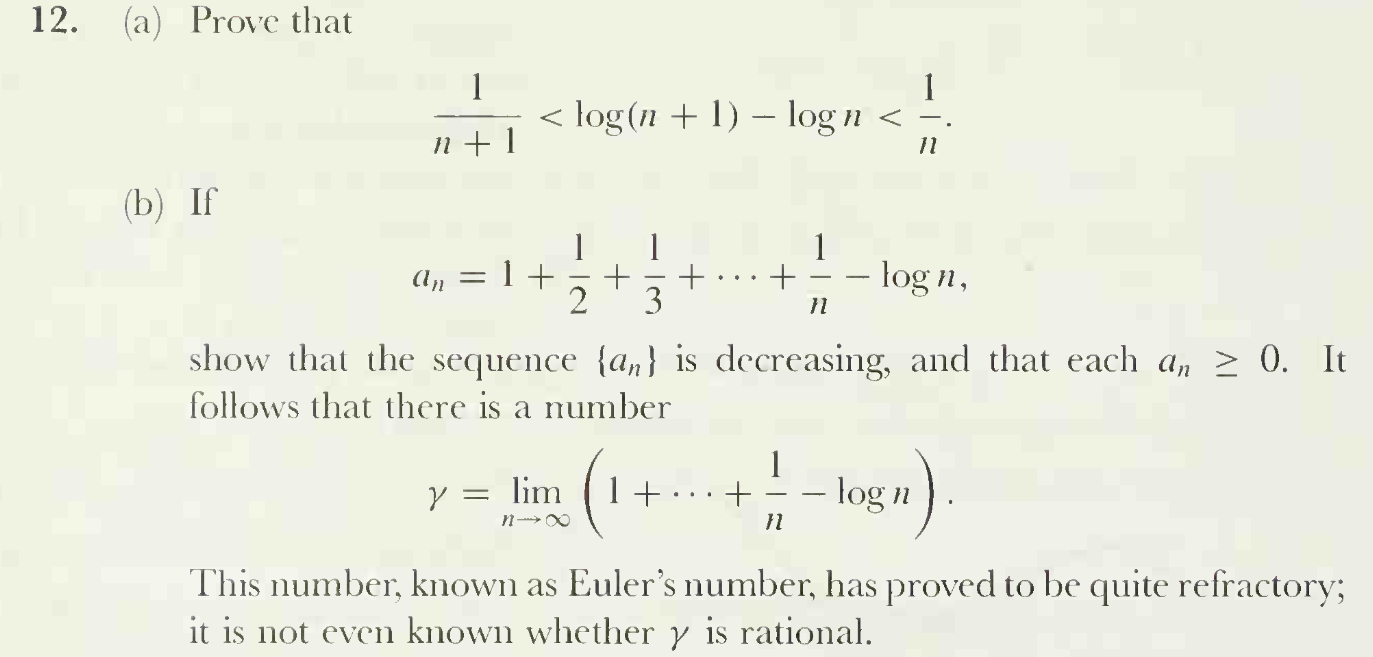
\includegraphics[width=\textwidth]{seq12}\\
\end{frame}


\end{document}
